% Subseccion Estructuras de control
\section{Estructuras de control}
Podemos clasificar cada una de las estructuras de control m�s comunes en programaci�n en uno
de los siguientes tipos:

\begin{itemize}
\item
\textbf{Secuencia:} Ejecuci�n sucesiva de una o m�s operaciones.
\item
\textbf{Selecci�n:} Se realiza una u otra operaci�n, dependiendo de una condici�n.
\item
\textbf{Iteraci�n:} Repetici�n de una o varias operaciones mientras se cumpla una condici�n.
\end{itemize}
\begin{figure}[H]
\begin{center}
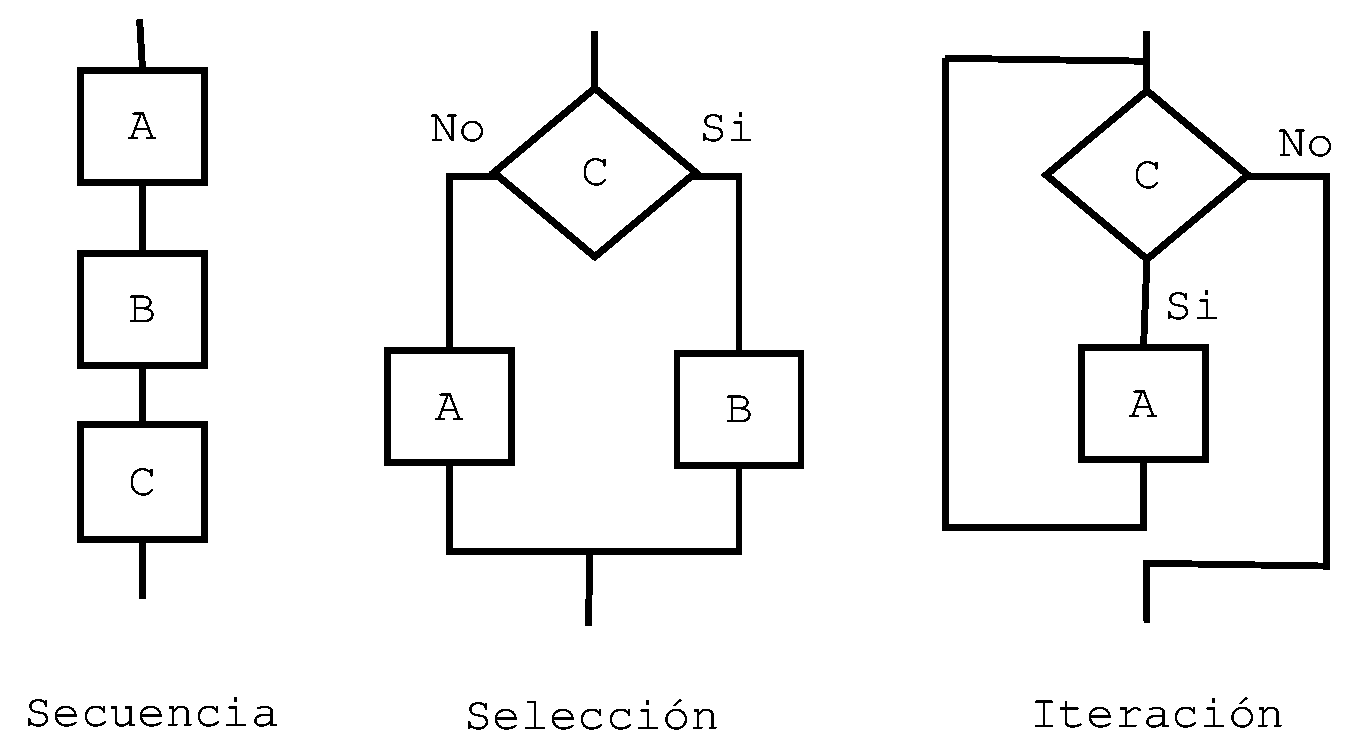
\includegraphics[width=8cm]{im/sintaxis/figura1.eps}
\end{center}
\end{figure}

\subsection{Sentencia if}
\begin{flushleft}
La forma general de esta sentencia es:
\end{flushleft}

\begin{verbatim}
if (expresion)
        sentencia
\end{verbatim}

\begin{figure}[H]
\begin{center}
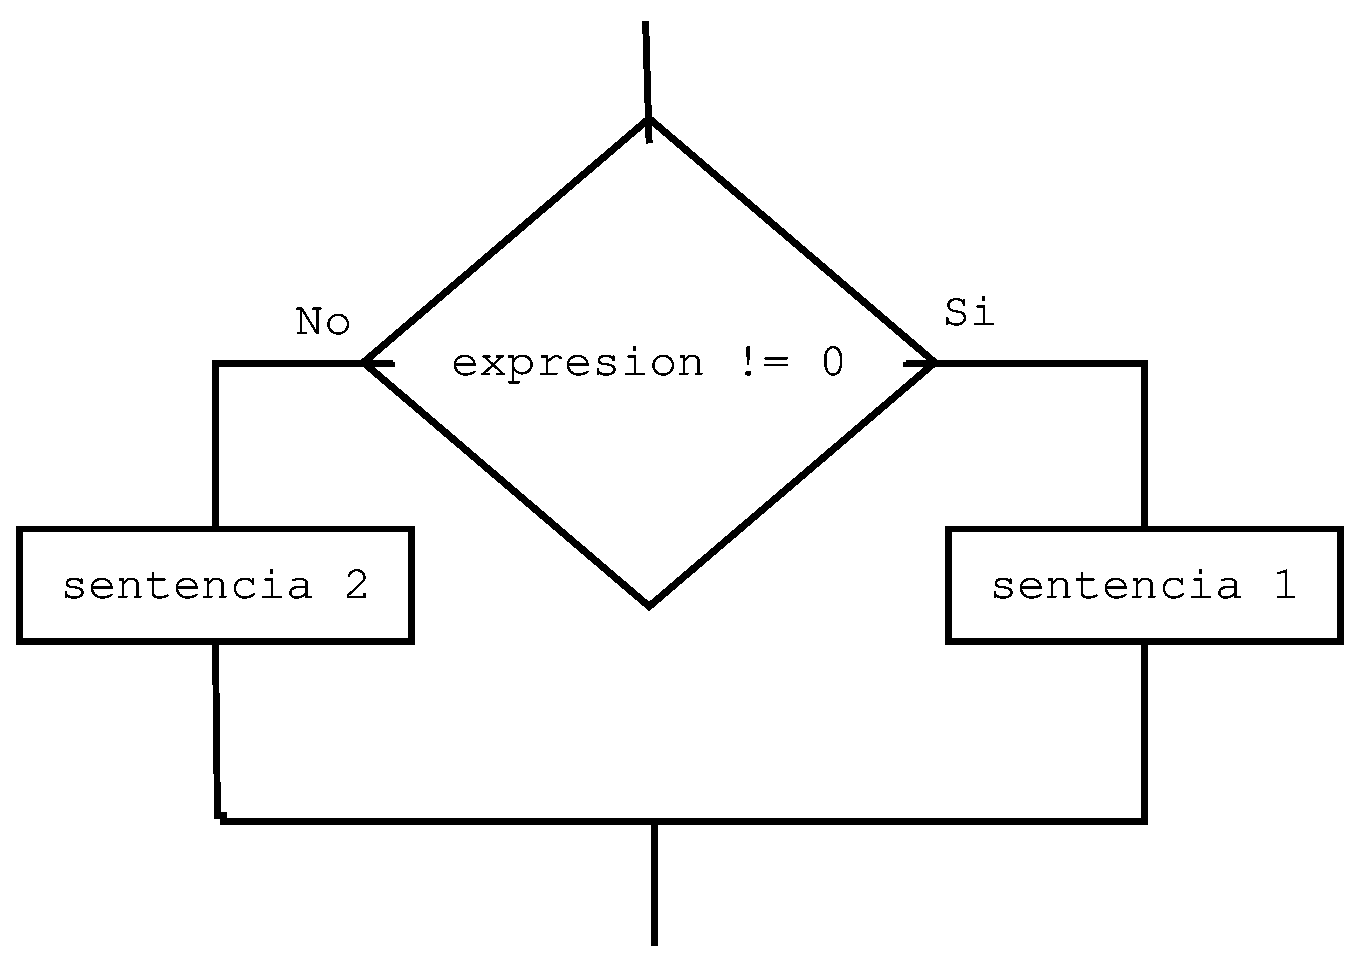
\includegraphics[width=6cm]{im/sintaxis/if.eps}
\caption{Sentencia if}
\end{center}
\end{figure}

\begin{itemize}
	
\item Si la \textbf{expresion} es verdadera (valor distinto de 0), entonces se ejecuta \textbf{sentencia}.
\item La \textbf{expresion} debe estar entre par�ntesis.
\item Si \textbf{sentencia} es compuesta tenemos:

\begin{verbatim}
if (expresion) 
{
        sentencia 1
        sentencia 2
              .
        sentencia N 
}
\end{verbatim}
 
\end{itemize}
\begin{flushleft}
Un ejemplo de uso de esta sentencia es el siguiente fragmento de programa, que decide si un n�mero es par:
\end{flushleft}

\begin{verbatim}
int numero = 0, esPar= 0;

if ((numero % 2) == 0)
        esPar = 1;
\end{verbatim}

\subsection{Sentencia if-else}

\begin{flushleft}
La forma general de esta sentencia es:
\end{flushleft}

\begin{verbatim}
if (expresion)
        sentencia 1
else
        sentencia 2
\end{verbatim}

\begin{figure}[H]
\begin{center}
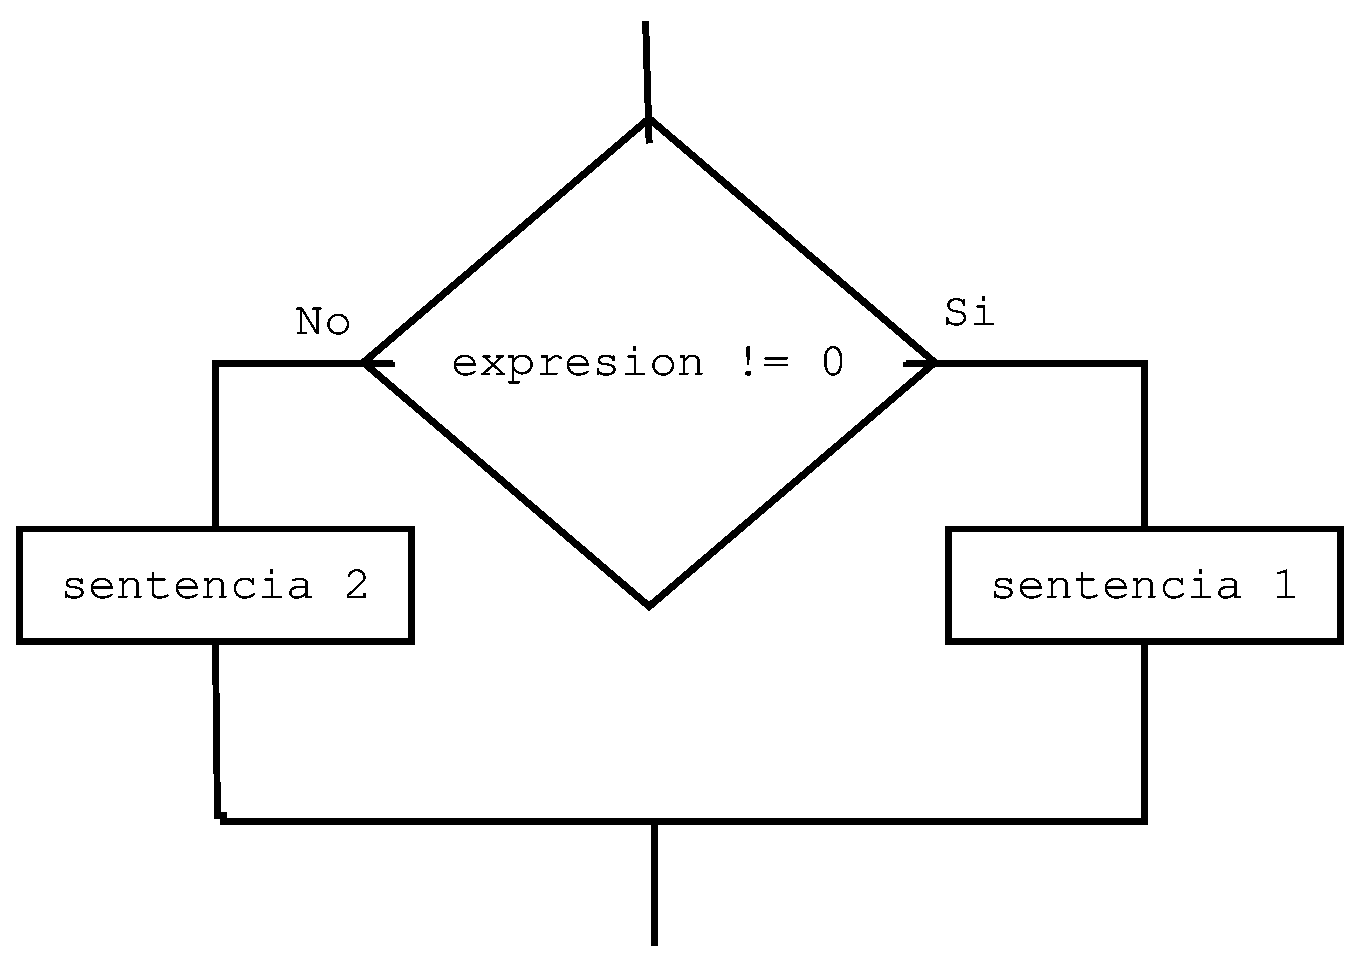
\includegraphics[width=8cm]{im/sintaxis/if-else.eps}
\caption{Sentencia if-else}
\end{center}
\end{figure}

\begin{itemize}
        
\item Si \textbf{expresion} es verdadera (valor distinto de 0), entonces se ejecuta \textbf{sentencia 1}; en caso contrario, se ejecuta \textbf{sentencia 2}.

\item Si las sentencias son compuestas se cierran entre \{ \}.

\item Las sentencias pueden ser a su vez sentencias \textbf{if-else}.

\begin{verbatim}
if (expresion 1)
    if (expresion 2)
        S1
    else
        S2
else
    S3
\end{verbatim}
\end{itemize}

\begin{flushleft}
Un ejemplo de uso de esta sentencia es el siguiente fragmento de programa, que elige el menor de tres n�meros:
\end{flushleft}

\begin{verbatim}
float a, b, c, menor;
a=2; b=4; c=1;

if (a < b) {
    if (a < c)
        menor = a;
    else
        menor = c;
} else {
    if (b < c)
        menor = b;
    else
        menor = c;
}
\end{verbatim}

\subsection{Sentencia switch}

\begin{flushleft}
La forma general de esta sentencia es:
\end{flushleft}

\begin{verbatim}
switch (expresion)
{
    case exp 1:
        sentencia 1;
        sentencia 2;
        break;

    case exp 2:
    case exp N:
        sentencia N;
        break;
    default:
        sentencia D;
}
\end{verbatim}

\begin{figure}[H]
\begin{center}
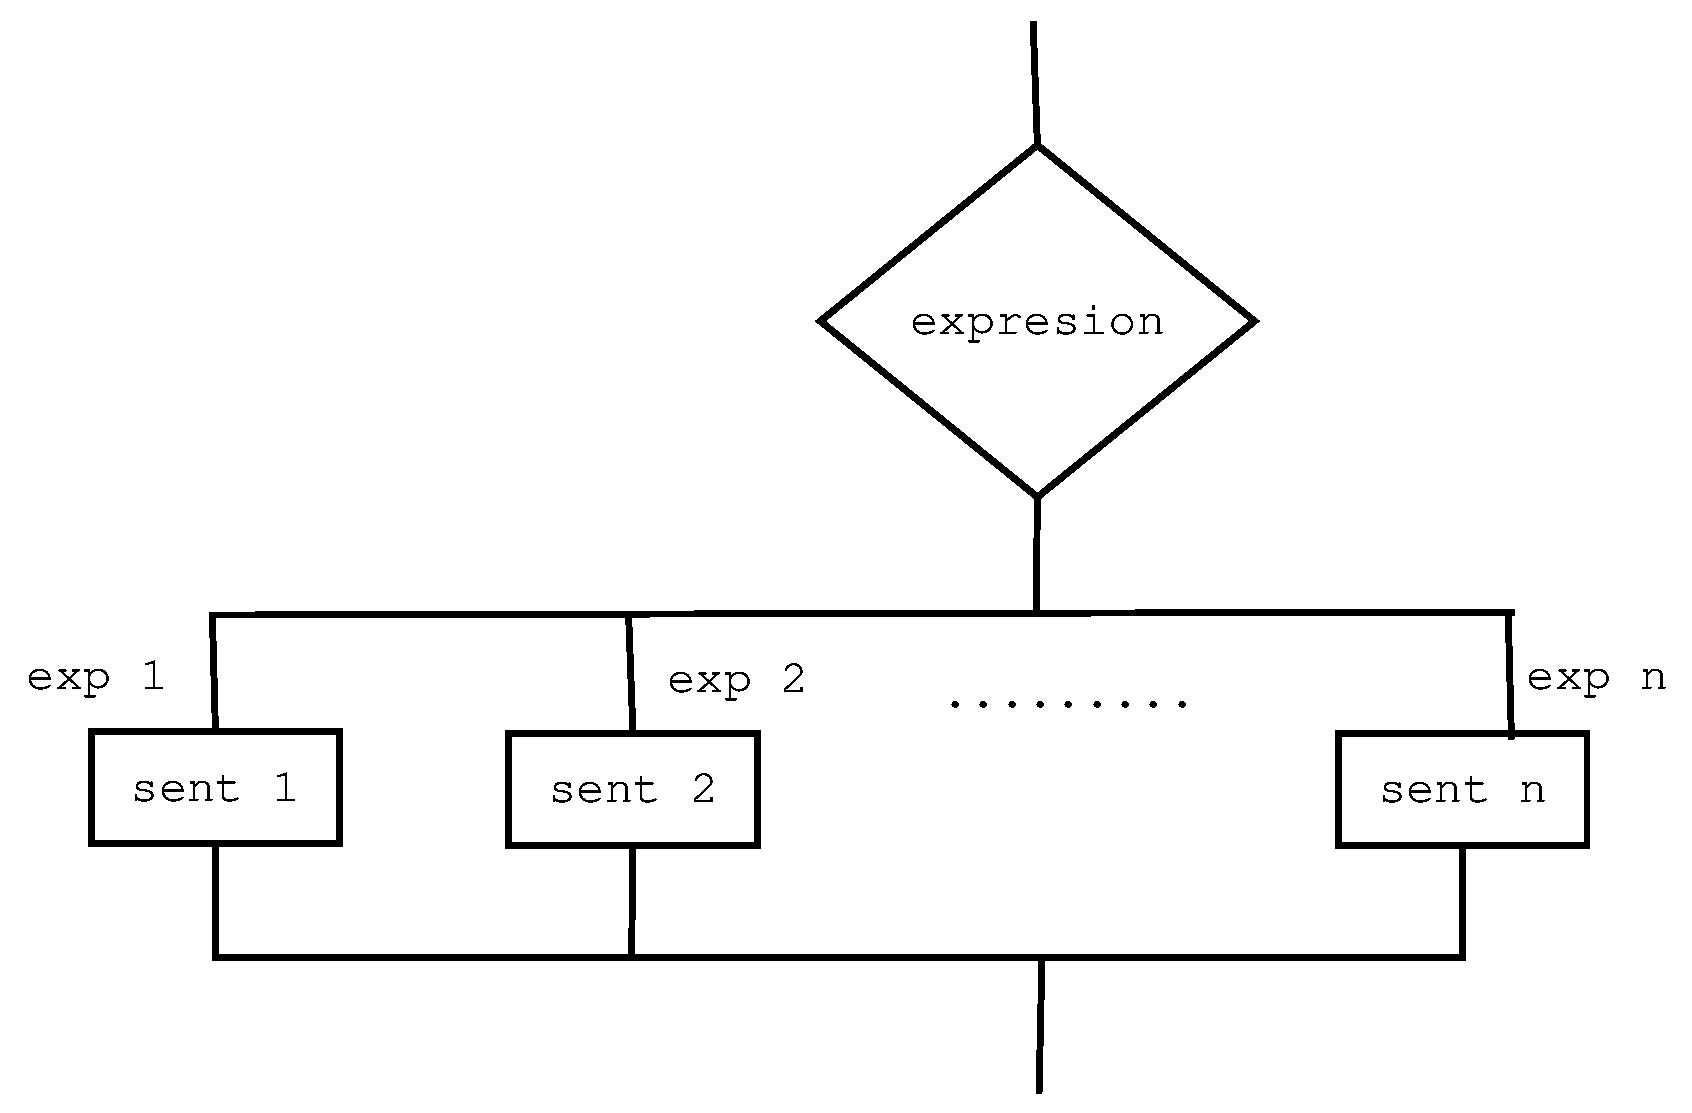
\includegraphics[width=10cm]{im/sintaxis/switch.eps}
\caption{Sentencia switch}
\end{center}
\end{figure}

\begin{itemize}
        
\item \textbf{expresion} devuelve un valor entero, pero tambi�n puede ser de tipo char.

\item \textbf{exp1}, ..., \textbf{exp N} representan expresiones constantes de valores enteros, 
aunque tambi�n pueden ser caracteres.


\end{itemize}



\begin{flushleft}
Un ejemplo de uso de esta sentencia es el siguiente fragmento de programa, que decide si imprime la vocal dada:
\end{flushleft}

\begin{verbatim}
letra='e';
switch(letra);
{
        case 'a': 
        case 'A': 
                printf(``Es la vocal a\n'');
                break;
        case 'e': 
        case 'E': 
                printf(``Es la vocal e\n'');
                break;
        case 'i': 
        case 'I':  
                printf(``Es la vocal i\n'');
                break;
        case 'o': 
        case 'O': 
                printf(``Es la vocal o\n'');
                break;
        case 'u': 
        case 'U': 
                printf(``Es la vocal u\n'');
                break;
        default: printf(``Es una consonante\n'');
}
\end{verbatim}


\subsection{Sentencia break}
La sentencia \textbf{break} se utiliza para terminar la ejecuci�n de
bucles o salir de una sentencia switch. Es necesaria en la sentencia
\textbf{switch} para transferir el control fuera de la misma. En caso
de bucles anidados, el control se transfiere fuera de la sentencia m�s
interna en la que se encuentre, pero no fuera de las externas.

\subsection{Sentencia for}
\begin{flushleft}
La forma general de esta sentencia es:
\end{flushleft}

\begin{verbatim}
for (expresion 1; expresion 2; expresion 3)
        sentencia;
\end{verbatim}

\begin{figure}[H]
\begin{center}
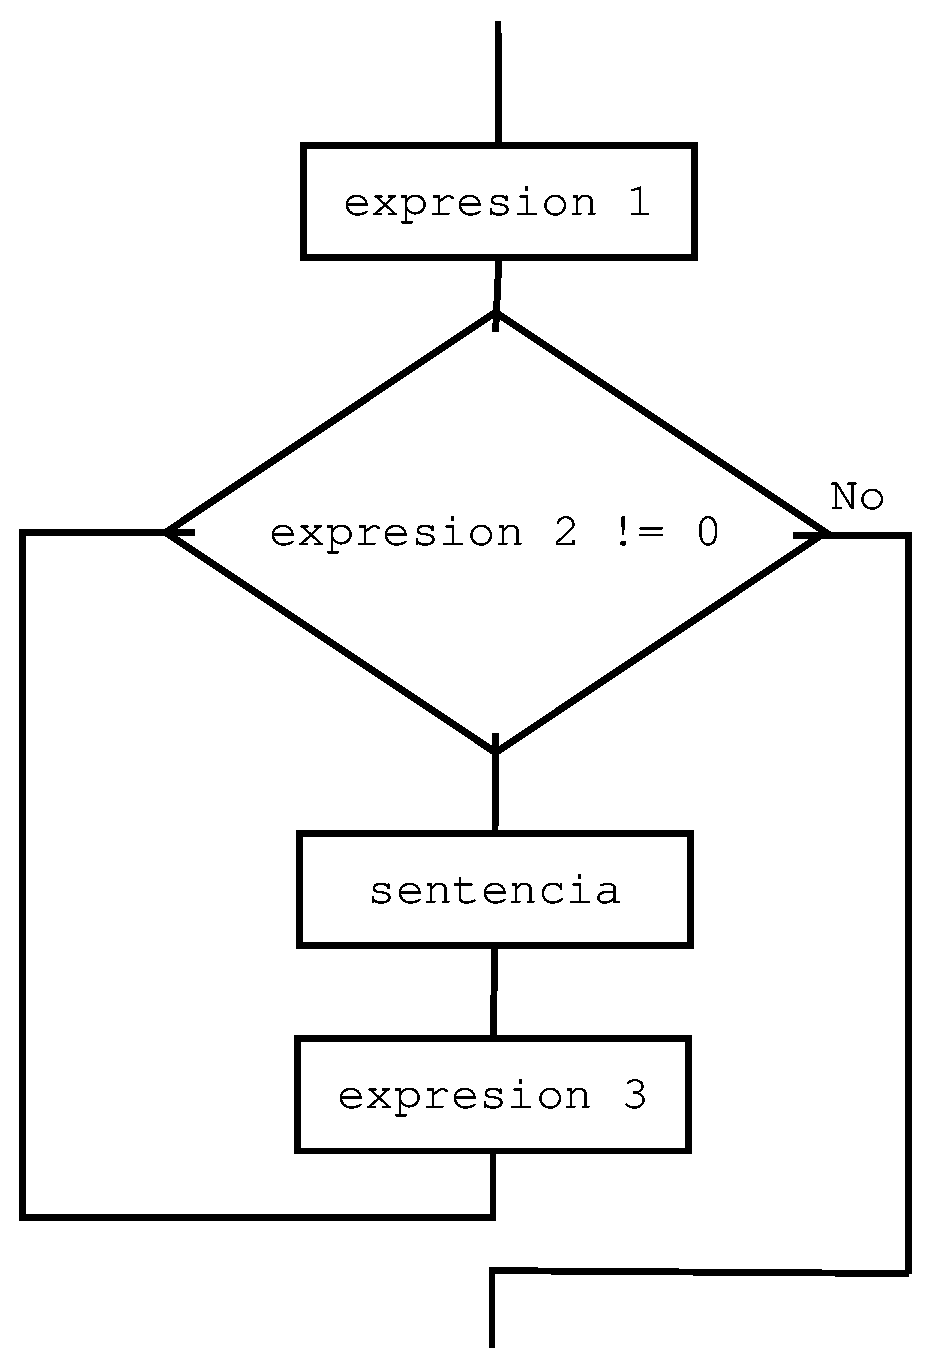
\includegraphics[width=55mm]{im/sintaxis/for.eps}
\caption{Sentencia for}
\end{center}
\end{figure}

\begin{itemize}
        
\item Inicialmente se ejecuta \textbf{expresion 1}, se hace para inicializar alg�n par�metro que controla la repetici�n del bucle.

\item \textbf{expresion 2} es una condici�n que debe ser cierta para que se ejecute \textbf{sentencia}.

\item \textbf{expresion 3} se utiliza para modificar el valor del par�metro.

\item El bucle se repite mientras \textbf{expresion 2} sea cierto.

\item Si \textbf{sentencia} es compuesta se encierra entre \{ \}.

\item Si se omite \textbf{expresion 2} se asumir� el valor permanente de 1 y el bucle se ejecutar� de forma indefinida (bucle infinito).
\end{itemize}

\begin{flushleft}
Un ejemplo de uso de esta sentencia es el siguiente fragmento de programa, que calcula la suma de los numeros del 1 al 100:
\end{flushleft}

\begin{verbatim}
int numero, suma;

suma=0;
for (numero=1; numero<=100; numero++)
    suma = suma + numero;  
\end{verbatim}

\subsection{Sentencia while}
\begin{flushleft}
La forma general de esta sentencia es:
\end{flushleft}

\begin{verbatim}
while (expresion)
        sentencia;
\end{verbatim}

\begin{figure}[H]
\begin{center}
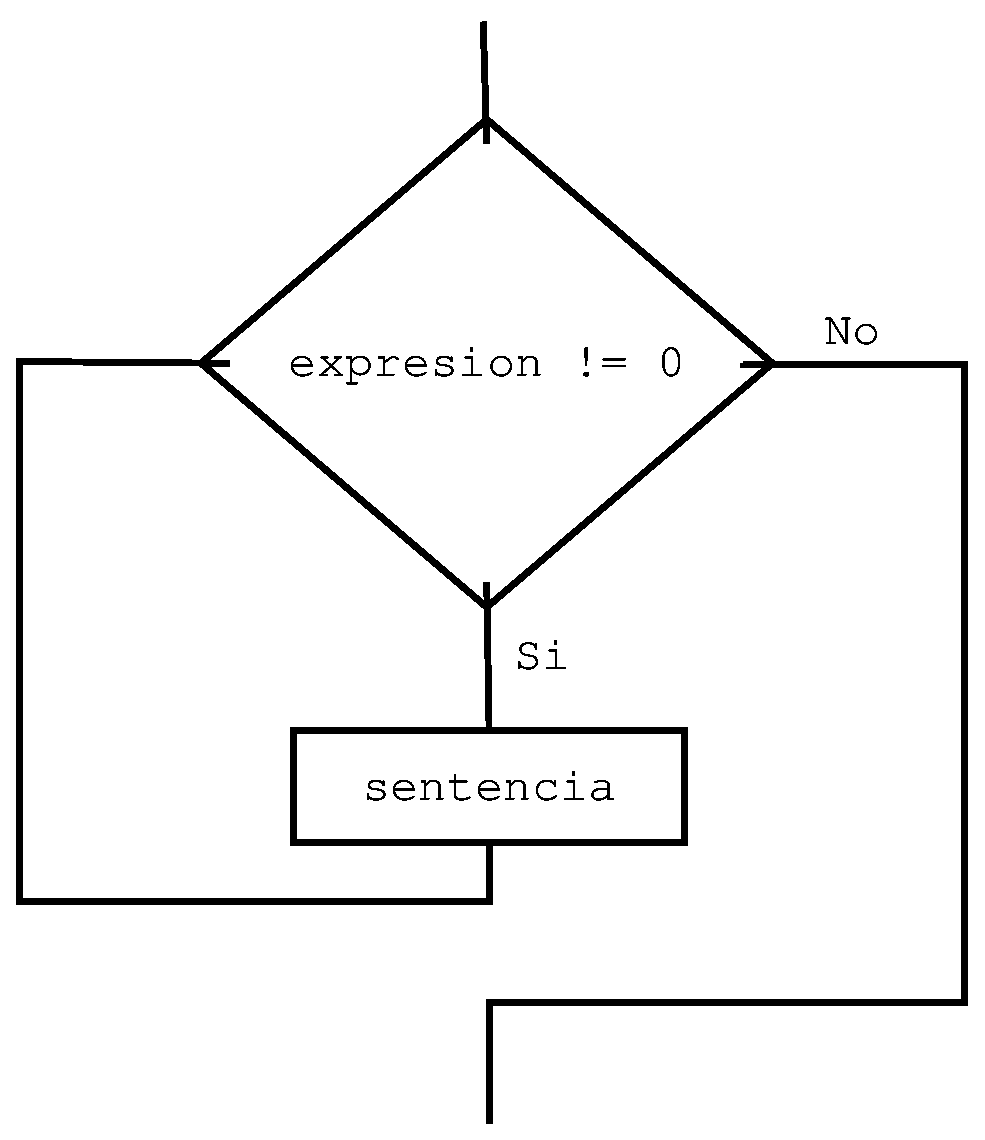
\includegraphics[width=62mm]{im/sintaxis/while.eps}
\caption{Sentencia while}
\end{center}
\end{figure}

\begin{itemize}
        
\item \textbf{sentencia} se ejecutar� mientras el valor de \textbf{expresion} sea verdadero.

\item Primero se eval�a \textbf{expresion}

\item Lo normal es que \textbf{sentencia} incluya alg�n elemento que altere el valor de \textbf{expresion} proporcionando as� la condici�n de salida del bucle.

\item Si \textbf{sentencia} es compuesta se encierra entre \{ \}.

\end{itemize}

\begin{flushleft}
Un ejemplo de uso de esta sentencia es el siguiente fragmento de programa, que calcula la suma de los numeros del 1 al 100:
\end{flushleft}

\begin{verbatim}
int suma, limite;

suma=1; limite=100;
while(limite>0)
{
    suma=suma+limite;
    limite--;
}
\end{verbatim}

\subsection{Sentencia do-while}
\begin{flushleft}
La forma general de esta sentencia es:
\end{flushleft}

\begin{verbatim}
do
    sentencia;
while (expresion);
\end{verbatim}


\begin{figure}[H]
\begin{center}
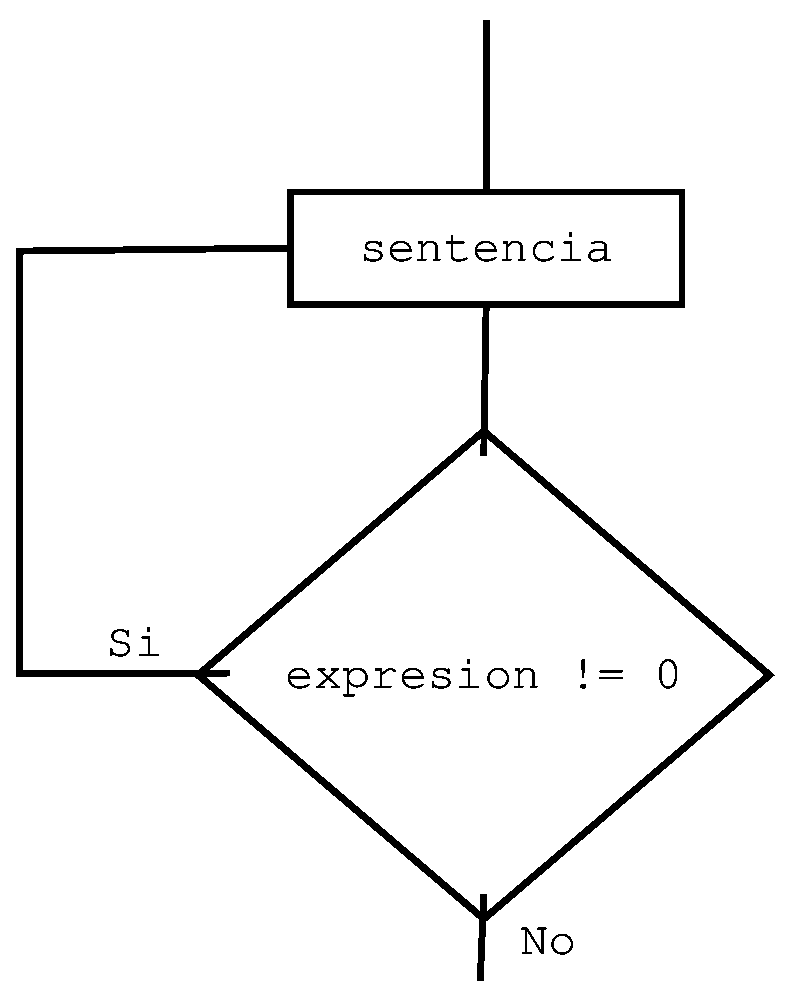
\includegraphics[width=50mm]{im/sintaxis/do-while.eps}
\caption{Sentencia do-while}
\end{center}
\end{figure}

\begin{itemize}
        
\item \textbf{sentencia} se ejecutar� mientras el valor de \textbf{expresion} sea verdadero.

\item \textbf{sentencia} siempre se ejecuta al menos una vez.
\item Si \textbf{sentencia} es compuesta se encierra entre \{ \}.

\end{itemize}

\nota{Lo normal es que \textbf{sentencia} incluya alg�n elemento que altere el valor de condici�n de salida del bucle.}

Para la mayor�a de las aplicaciones es mejor y m�s natural comprobar la condici�n antes de ejecutar el bucle, por ello se usa m�s la sentencia \textbf{while}.\\

\begin{flushleft}
Un ejemplo de uso de esta sentencia es el siguiente fragmento de programa, que pide un n�mero igual a 0:
\end{flushleft}

\begin{verbatim}
int numero = 0;
do
{
        printf("Introduce el n�mero 0:\n");
        scanf("%d", &numero); /* Se lee el numero */
} while (numero != 0);
\end{verbatim}
